\documentclass[12pt,a4paper]{article}

\usepackage[T1]{fontenc}
\usepackage[utf8]{inputenc}
\usepackage[margin=2.5cm]{geometry}
\usepackage{graphicx}
\usepackage[hidelinks]{hyperref}
\usepackage{fancyhdr}
\usepackage{lastpage}
\usepackage{appendix}
\usepackage{color}
\usepackage{palatino}
\usepackage{changepage}
\usepackage{subcaption}
\usepackage{enumitem}
\usepackage{csquotes}
\usepackage{verbatim}
\usepackage{minted}
\usepackage{listings}
\usepackage[ruled,vlined]{algorithm2e}

\usemintedstyle{fruity}

\definecolor{mygreen}{rgb}{0,0.6,0}
\definecolor{mygray}{rgb}{0.5,0.5,0.5}
\definecolor{mymauve}{rgb}{0.58,0,0.82}

\lstset{
  backgroundcolor=\color{white},   % choose the background color; you must add \usepackage{color} or \usepackage{xcolor}; should come as last argument
  basicstyle=\ttfamily,        % the size of the fonts that are used for the code
  breakatwhitespace=false,         % sets if automatic breaks should only happen at whitespace
  breaklines=true,                 % sets automatic line breaking
  captionpos=b,                    % sets the caption-position to bottom
  commentstyle=\color{mygreen},    % comment style
  deletekeywords={...},            % if you want to delete keywords from the given language
  escapeinside={\%*}{*)},          % if you want to add LaTeX within your code
  extendedchars=true,              % lets you use non-ASCII characters; for 8-bits encodings only, does not work with UTF-8
  frame=single,                    % adds a frame around the code
  keepspaces=true,                 % keeps spaces in text, useful for keeping indentation of code (possibly needs columns=flexible)
  keywordstyle=\color{blue},       % keyword style
  %language=Octave,                 % the language of the code
  morekeywords={*,...},            % if you want to add more keywords to the set
  numbers=left,                    % where to put the line-numbers; possible values are (none, left, right)
  numbersep=5pt,                   % how far the line-numbers are from the code
  numberstyle=\tiny\color{mygray}, % the style that is used for the line-numbers
  rulecolor=\color{black},         % if not set, the frame-color may be changed on line-breaks within not-black text (e.g. comments (green here))
  showspaces=false,                % show spaces everywhere adding particular underscores; it overrides 'showstringspaces'
  showstringspaces=false,          % underline spaces within strings only
  showtabs=false,                  % show tabs within strings adding particular underscores
  stepnumber=2,                    % the step between two line-numbers. If it's 1, each line will be numbered
  stringstyle=\color{mymauve},     % string literal style
  tabsize=2,                       % sets default tabsize to 2 spaces
  title=\lstname                   % show the filename of files included with \lstinputlisting; also try caption instead of title
}

\title{Binary Space Partitions}
\author{Carlos Requena López}

%% Fancy layout
\pagestyle{fancy}
\lhead{Binary Space Partitions}
\chead{}
\rhead{}
\lfoot{}
\cfoot{}
\rfoot{Page \thepage\ of \pageref{LastPage}}
\renewcommand{\headrulewidth}{0.4pt}
\renewcommand{\footrulewidth}{0.4pt}


%%% --- %%% --- DOCUMENT START --- %%% --- %%%
\begin{document}
\maketitle
\thispagestyle{empty}
\tableofcontents
\newpage
%%% Counting pages now %%%
\pagestyle{fancy}
\setcounter{page}{1}


\section{Introduction}

This first assignment deals with recursive autopartitioning of a two
dimensional space. Autopartitions, in contrast to partitions, are
performed extending the supporting lines of the segments already
present on the plane.

In particular, with partitions in general, we stop executing the
algorithm when there is

Having direct application in computer graphics, the most interesting
parameter when considering these partitions in the size of the
generated tree, since that's what is used in practice to decide what
to render first in the scene of a computer screen.

\section{Analysis and expectations}

We define the algorithm RandAutopart in \ref{algo}

\begin{algorithm}[h]
  \SetAlgoLined
  \KwIn{A set S of segments}
  \KwOut{The autopartition binary tree}

  \nl Pick a random permutation of S and take the first element\;
  \nl Extend this element into a line and create a node with it in the tree\;
  \nl Filter the segments strictly to the left in the \texttt{left}
  child\;
  \nl Filter the segments strictly to the right in the \texttt{right}
  child\;
  \nl \For{segment in all segments that intersect}{
    \nl add its subsegment laying on the left part to the
    \texttt{left} child\;
    \nl add its subsegment laying on the right part to the
    \texttt{right} child\;
  }
  \nl \While{\texttt{left} or \texttt{right} have segments in them}{
    \nl Repeat this procedure recursively on both sets\;
  }
\caption{\bf RandAutopart}
\label{algo}
\end{algorithm}

The upper bound found in literature \cite{Motwani:1995:RA:211390},
corresponds to the upper bound of the random algorithm for any
input. The expectation would be for this boundary to be closer when
choosing the worst possible input (segment positioning wise) and
further away when adding randomness to the input and even more when
giving the the most trivial input possible: parallel segments, in
which case the number of partitions would be $n+1$.

The algorithm will be therefore tested with a random input and a
crafted, ``evil'' input, to try and get close to this upper bound
without ever exceeding it.

\section{Implementation}

$n$ disjoint segments are generated and placed on a $H\times W$
canvas, where $H$ is the height and $W$ the width, both in pixels.

The first element of a random permutation of those $N$ segments is
taken, its supporting line extended, and the host space (the plane)
partitioned in two. The same procedure is applied recursively to

In order to know which segments another line intersects, some
primitive geometry operations have to be implemented. Since this is
done from scratch however, we expect them to not be as robust as the
ones some external library could provide. These operations include:

\begin{itemize}
\item Testing to which side a point is with respect to a line segment
  (of if it is on the line).
\item Testing whether a segment is on one side or the other of a
  segment (or if it is colinear).
\item Testing whether a segment could potentially intersect another if
  its supporting line is extended.
\item Testing whether two segments intersect each other.
\item Determining the coordinates of the intersection of a line and a
  segment.
\end{itemize}

Most operations rely of calculating the orientation determinant for
the line segment defined by two points and a third.

The generated segments' coordinates are integers to begin with and
Clojure uses a \texttt{Ratio} type to make arithmetic calculations as
exact as possible at the expense of performance, which is not an
issue.

In addition to this, this implementation tries to handle degenerate
and special cases as much as possible (colinear segments,
segment-on-segment, vertical segments, out-of-bounds segments, segment
of size 0 - a point, etc).

For example, for the input shown in figure \ref{fig:sample-input} the
corresponding partition tree is the following (there are no
intersections in this case):

\begin{lstlisting}[frame=single]
"BSpace partitions"
{:seg {:a {:x 492, :y 556}, :b {:x 388, :y 932}},
 :left
 {:seg {:a {:x 625, :y 409}, :b {:x 530, :y 745}},
  :left (),
  :right
  {:seg {:a {:x 626, :y 355}, :b {:x 588, :y 243}},
   :left (),
   :right ()}},
 :right
 {:seg {:a {:x 264, :y 626}, :b {:x -8, :y 571}},
  :left (),
  :right
  {:seg {:a {:x 88, :y 291}, :b {:x 36, :y 79}},
   :left (),
   :right ()}}}
\end{lstlisting}

\begin{figure}[ht!]
  \centering
  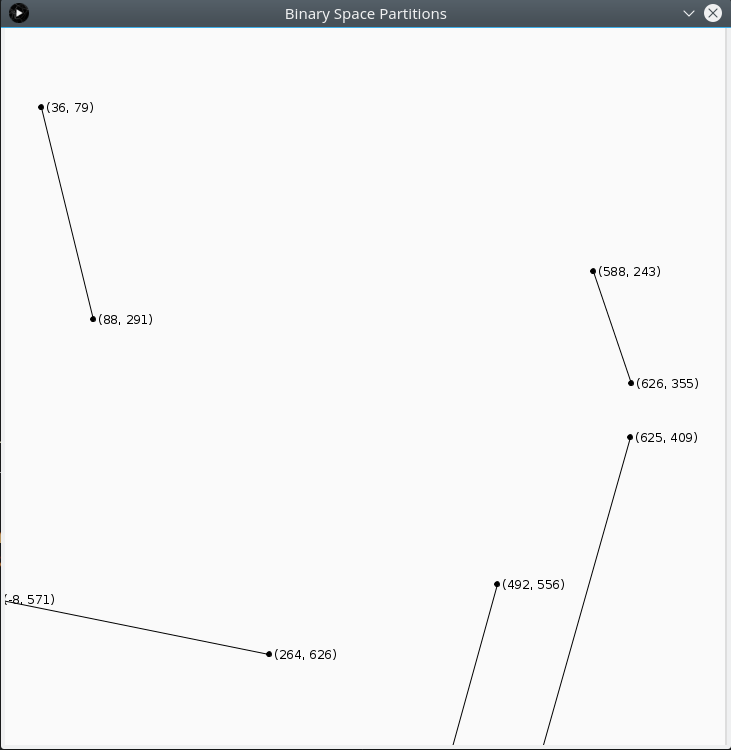
\includegraphics[width=0.7\textwidth]{img/sample-input.png}
  \caption{Five random segments on a 720x720 canvas}
  \label{fig:sample-input}
\end{figure}


\section{Results}

\section{Conclusion}

% \begin{figure}[ht!]
%   \centering
%   \includegraphics[width=1\textwidth]{some_graphic.png}
%   \caption{}
%   \label{fig:fig1}
% \end{figure}

\appendix
\section{Appendix - code listing}

\begin{minted}{clojure}
\end{minted}

\nocite{*}
\bibliographystyle{plain}
\bibliography{refs}

\end{document}
